\documentclass[tikz,border=8pt]{standalone}
\usepackage[T1]{fontenc}
\usepackage{lmodern}
\renewcommand{\familydefault}{\sfdefault}
\usetikzlibrary{positioning,arrows.meta,calc}

\tikzset{
  branch/.style={draw, dashed, rounded corners=2pt, align=center, font=\small\sffamily,
    fill=white, inner sep=4pt, minimum height=9mm, text width=78mm},
  note/.style={font=\scriptsize\sffamily, align=center, text width=78mm, inner sep=1pt},
  lbl/.style={font=\scriptsize\sffamily, fill=white, inner sep=1pt, align=center}
}

\begin{document}
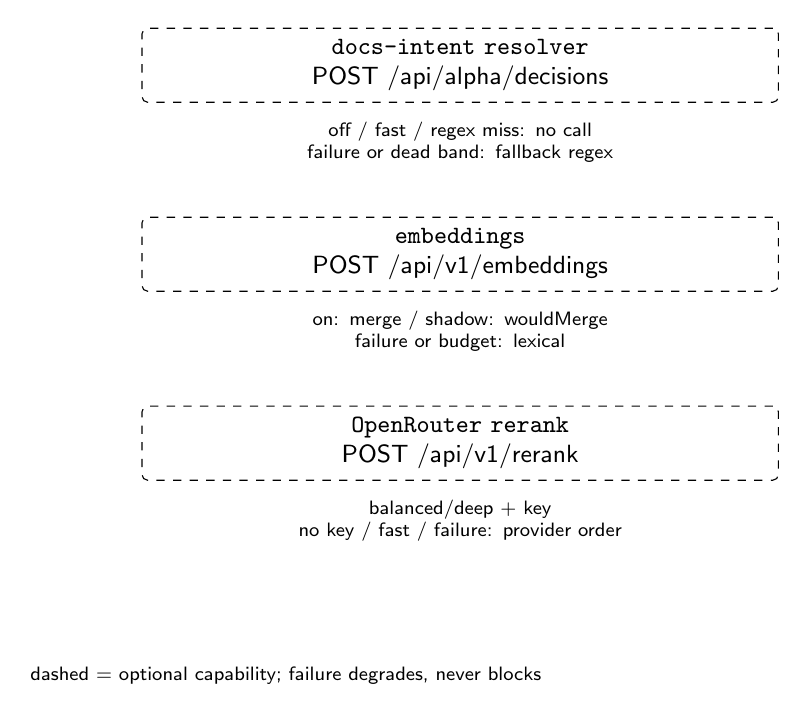
\begin{tikzpicture}
\node[branch] (dec) at (0,5.2) {\texttt{docs-intent resolver}\\POST /api/alpha/decisions};
\node[note, below=2mm of dec] (decnote) {off / fast / regex miss: no call\\failure or dead band: fallback regex};

\node[branch] (emb) at (0,2.8) {\texttt{embeddings}\\POST /api/v1/embeddings};
\node[note, below=2mm of emb] (embnote) {on: merge / shadow: wouldMerge\\failure or budget: lexical};

\node[branch] (rer) at (0,0.4) {\texttt{OpenRouter rerank}\\POST /api/v1/rerank};
\node[note, below=2mm of rer] (rernote) {balanced/deep + key\\no key / fast / failure: provider order};

\node[lbl, anchor=north west, fill=none] at (-5.5,-2.4) {dashed = optional capability; failure degrades, never blocks};
\end{tikzpicture}
\end{document}